Galant is based on GDR, which we discuss in Section~\ref{sec:gdr_features}.
We then give an overview of Galant -- Section~\ref{sec:galant_overview}.
The most important aspect of Galant is the ability to create animations easily,
as discussed in Section~\ref{sec:animator}.
Then we give a brief overview of the user interface in Section~\ref{sec:user_interface}.
More detailed documentation is in the Appendices --
Appendix~\ref{sec:animations} for animation examples,
\ref{sec:user_documentation} for user documentation,
\ref{sec:programmer_guide} for animation programmer documentation,
and \ref{sec:bugs} for known bugs.

\subsection{GDR: Galant's predecessor}
\label{sec:gdr_features}
Galant is a successor to
GDR~\cite{1991-TR_NCSU_CSC-Stallmann,1992-CSDM-Stallmann} and has much of the
same functionality.
The design of GDR is illustrated in Fig.~\ref{fig:gdr}.
To the left of the dotted line are the interactions with external entities,
as supported by GDR.
The GDR user, when running a specific animation created and compiled
externally, acts as both the editor of problem instances and as initiator of an
algorithm animation with which (s)he may then interact, i.e., plays the role
of explorer and of observer. 
Input and output take the form of a simple text-based file format that can be
manipulated outside of GDR via text filters, graph editors, graph drawing
applications, etc. It is this external manipulation capability
that makes GDR a tool rather than a
closed system.

The animation creator writes a C program that interacts with a graph ADT
whose functions access and/or modify both the internal representation of the
graph and the user's view of it. The ADT functions can be classified into one
of three categories depending on the graph attributes accessed:
(i)~\emph{logical} attributes --- labels (and identities) of nodes and labels
and endpoints of edges; (ii)~\emph{geometric} attributes --- the positions of
nodes and labels and
inflection points of edges; and (iii)~\emph{display} attributes ---
highlighting of nodes and edges, making labels visible/invisible, etc. 

\begin{figure}

\begin{center}
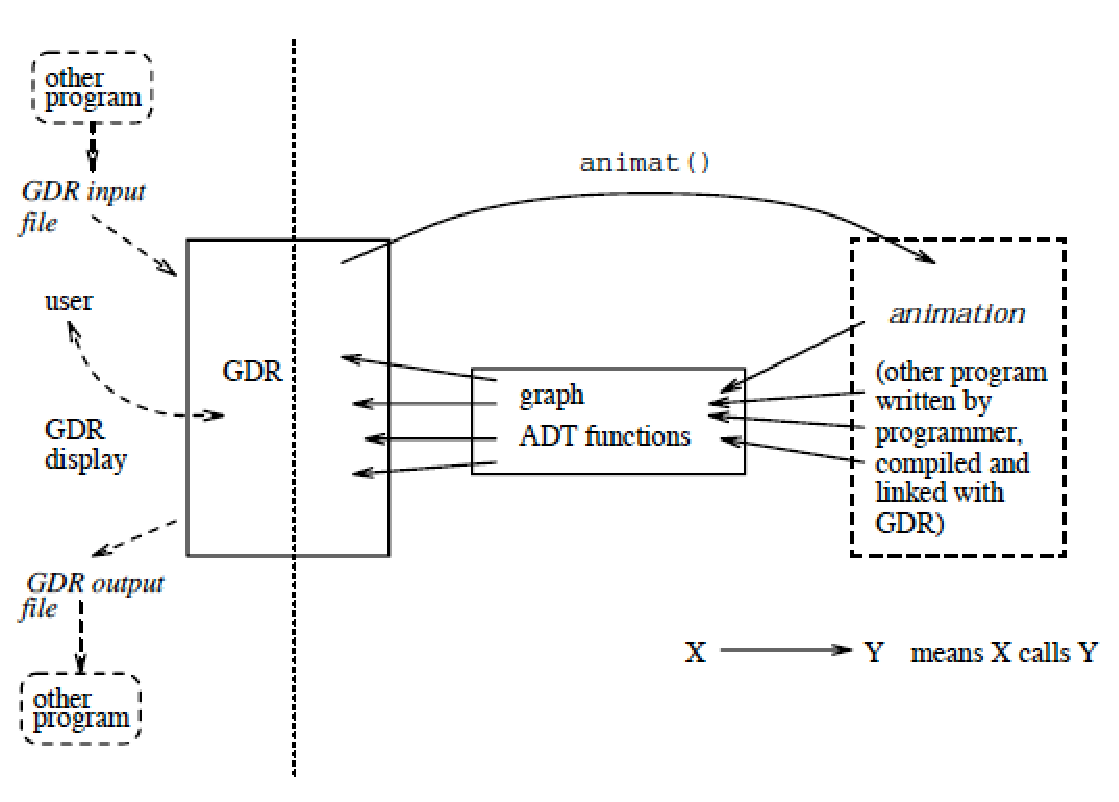
\includegraphics[scale=0.6]{X_gdr_design}
\end{center}

\caption{GDR design.}
\label{fig:gdr}
\end{figure}

While GDR has much to recommend it when compared with other algorithm
animation software, it suffers from some serious drawbacks:

\begin{itemize}
\item
  Each animation is a separate C program that interacts with an X11 window
  server.
  Therefore GDR is not portable.
  %% It is not possible to load (and apply) more than one animation to
  %% the same graph.
\item
  The user interface is crude. Aside from being black and white it has no
  file browser, no rubber-banding of moves, non-standard keyboard shortcuts
  and an unappealing look and feel.
%% \item
%%   The format for storing graphs, while simple and text-based, does not
%%   resemble any other graph format and is difficult to edit or filter.
\item
  While the API supports access to the graph itself, there is no API support for
  data structures commonly used in graph algorithms (stacks, queues, priority
  queues).
\end{itemize}

% [Last modified: 2013 06 25 at 14:51:36 GMT]


\begin{figure}[p]

\begin{center}
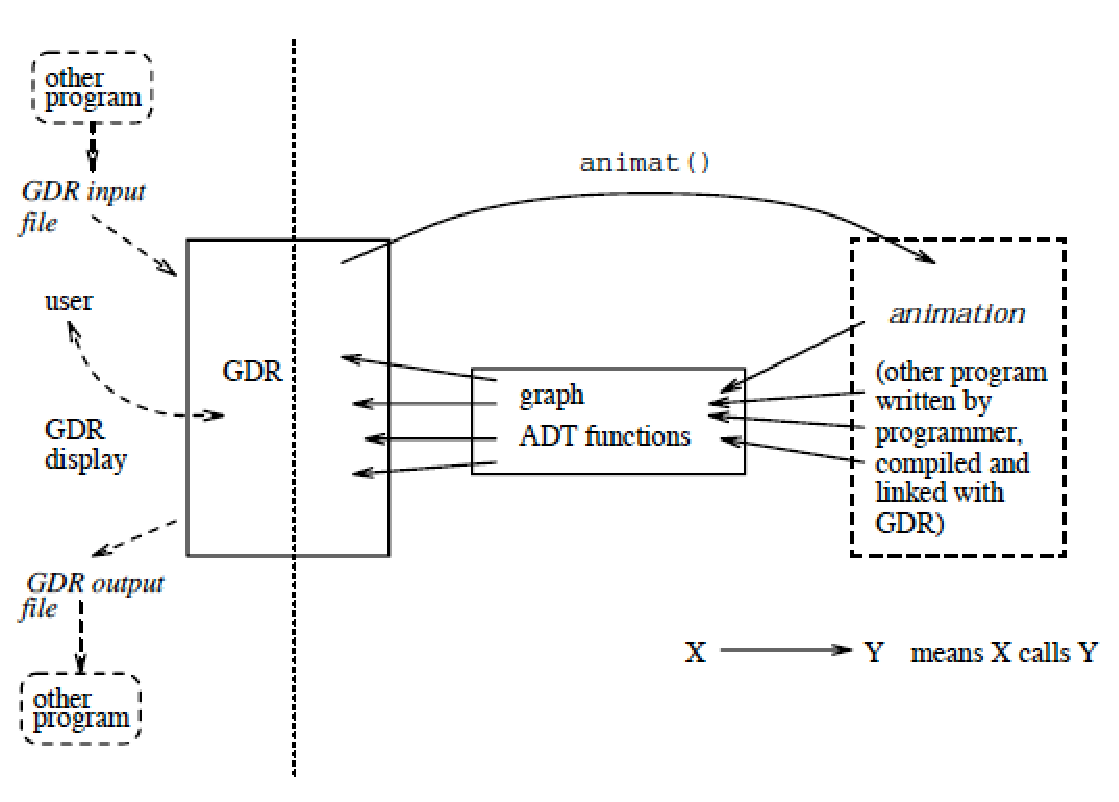
\includegraphics[scale=0.6]{X_gdr_design}
\end{center}

\caption{GDR design.}
\label{fig:gdr}
\end{figure}

\begin{figure}

\centering

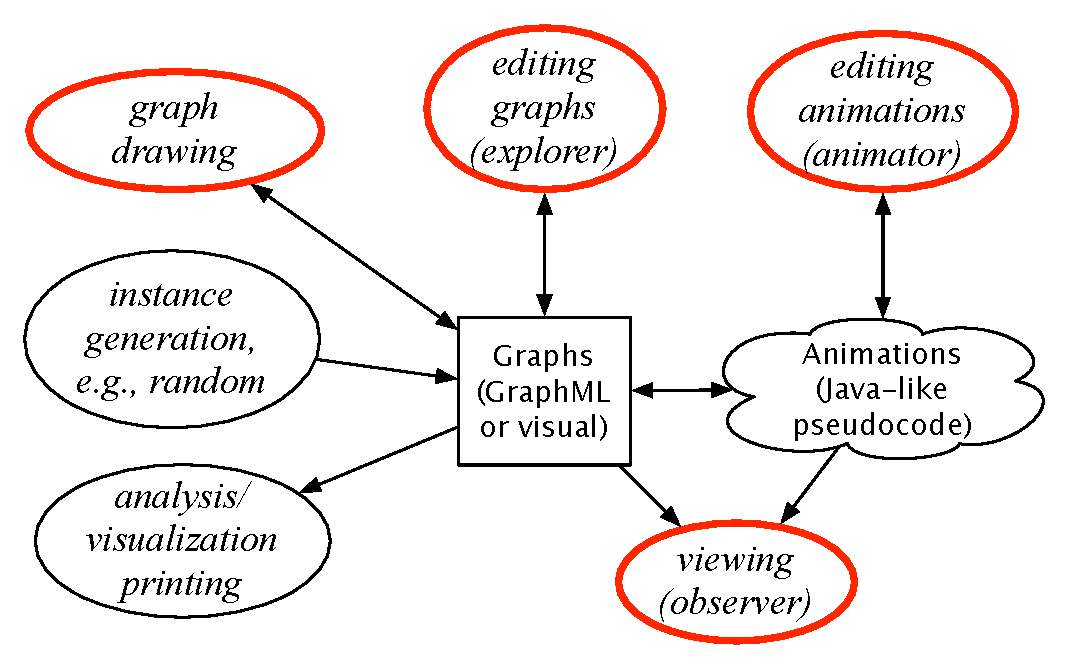
\includegraphics[width=\columnwidth]{X_overview_diagram}

\caption{Illustration of Galant design and functionality. Arrows indicate
  data flow. All functions, shown as ovals can be performed easily outside of
Galant. The ones with thick red borders are part of current Galant
functionality.}

\label{fig:overview_diagram}
\end{figure}

% [Last modified: 2013 06 25 at 16:04:45 GMT]


\subsection{Galant overview}
\label{sec:galant_overview}
Fig.~\ref{fig:overview_diagram} gives an overview of Galant functionality.
A graphical user interface (GUI) allows the user to edit both graphs and
algorithm animations, either loaded as already existing files or newly
created. At any point, the user can apply a selected animation to a selected
graph for viewing.
The animation program 
steps forward until it
displays the next animation event or, if a \texttt{beginStep()}
call has marked the start of a sequence of events, until
it reaches the next \texttt{endStep()} call.
It then pauses execution and waits for the user to decide whether to
step forward, step backward, or exit.
A step forward resumes execution while a step backward returns the display to a previous
state.
The algorithm resumes execution only when the \emph{display state}
indicated by the user's sequence of forward and backward steps
($f-b$, where $f$ is the number of forward and $b$ the number of backward steps)
exceeds the \emph{algorithm state}, the number of animation steps the algorithm
has executed.

When editing a graph the user can create/delete nodes and edges (when in the appropriate mode)
by clicking and/or
moving the mouse, and can move vertices by dragging the mouse.
There is also an interface for specifying labels, weights and colors for both
nodes and edges.
Keyboard shortcuts are available for these operations.
 
A preferences panel allows the user to select font size for labels and a
variety of other options.
Any changes to a graph are also reflected in a text (GraphML) representation
of the graph, which can also be edited directly. Naturally the GraphML
representation can also be created or edited externally: by a random or
structured graph generator, by translation from another format, by directly
editing the GraphML or by invoking a separate graph editor.
Galant has a built-in force-directed drawing program 
(see Hu~\cite{2006-Mathematica-Hu}) to position nodes
automatically if so desired.
Automatic drawing is useful when the input GraphML file does not provide position
information for the nodes (and their positions are selected randomly).
Other drawing programs, such as those provided by GraphViz~\cite{GraphViz}
and the huge body of research carried on by the graph drawing community~\cite{graph_drawing},
can be used externally as well.
Graphs used in Galant animations
can be analyzed externally using tools such as Gephi~\cite{gephi}.

Editing/compiling an algorithm animation is just like performing the same
operations on a Java program.
The compiler is essentially a Java
compiler that preprocesses the algorithm code
and compiles it, importing the relevant modules.
The preprocessor converts traversals of incidence lists and other
lists of nodes or edges into the corresponding, more obscure, Java code.
It also shields the Galant programmer from such syntactic circumlocutions
as declaring \texttt{static} methods.
Almost all Galant functions are available as both methods
using object-oriented notation, e.g., \texttt{v.highlight()},
and as procedures, e.g., \texttt{highlight(v)}.

Because the functionality of the Galant editor is limited, it is usually more
convenient to use an external program editor, reserving the Galant editor to
make minor changes in response to compile-time or runtime errors.

We use GraphML~\cite{GraphML} as our graph representation because it is
flexible, it can easily be extended, and parsers, viewers and translation
tools are becoming more common.  Because GraphML is specialized XML, parsers
for the latter, based on the Document Object Model (DOM) can be used. These
are available for many programming languages.  Translators to other formats
are also available or can easily be constructed.  For example, the
GraphViz~\cite{GraphViz} download provides one; unfortunately it preserves
only the connectivity information.  However, there is straightforward mapping
between the GraphML attributes we use (positions of nodes and colors, etc.,
of nodes and edges) and the corresponding ones in GraphViz format.  We have
written conversion scripts among the following formats: GraphML,
gml~\cite{1999-TRPassau-Himsolt}, sgf
(used for layered graphs in crossing minimization), and dot (GraphViz~\cite{GraphViz}).

% [Last modified: 2013 06 25 at 18:06:12 GMT]


\subsection{For the animator}
\label{sec:animator}
When it comes
to creating animations,
Galant offers the most significant advantages over GDR and, a fortiori,
over other algorithm animation software. Among these are:

\begin{itemize}

\item
  The API interface is simpler, due, in part, to the fact that the
  underlying language is Java rather than C.

\item
  Each node and edge has both a weight and a label. Conversion of a weight to
  a number is automatic while labels are kept as text. The programmer can
  choose the appropriate attribute, which makes the implementation more
  transparent and devoid of explicit conversions.

\item
  Most data structures are built in: stacks, queues, lists and priority
  queues of both edges and vertices. Priority queues implicitly use the
  weight attribute of the node/edge in question. The weight attribute is also
  used for sorting.

\item
  An algorithm initially designed for directed graphs can usually be applied
  to undirected graphs (and get the desired interpretation) with no change in
  the implementation.
  This is useful, for example, when implementing Dijkstra's
  algorithm.

\item
  The interface that allows an explorer to edit graph instances can also be used
  to edit, compile, and run algorithm implementations. While initial creation
  and major edits are usually more convenient via a standard program editor
  offline, an algorithm window in Galant can be used to view the algorithm and
  make corrections in response to compile or runtime errors.

\end{itemize}

The philosophy behind the API design is that it should be usable by someone
familiar with graph algorithms but only a rudimentary knowledge of Java (or
any other programming language).
The fact that Galant code resembles the pseudocode used
in one of the most
popular algorithm design and analysis texts, that of Cormen et al.~\cite{2009-Intro_to_Algorithms-Cormen},
attests to the fact that we have succeeded.

A key advantage of the API design, not present in, for example, BALSA or Edgy,
is that it sits directly on top of Java.
This allows the animator to develop arbitrarily complex algorithms using other Java class API's and ones devised by the animator.
More importantly, it allows Galant to offer significant new functionality
provided by developers with only a modicum of Java training:
\emph{sets} of nodes and edges (in addition to the stacks and queues already
built in)\footnote{
  The most recent release has sets built-in -- these were easily added by the
  developers.
}
or significant infrastructure for algorithms in a specific domain,
as was done for crossing minimization in layered graphs.


%\subsection{For the explorer}
\label{sec:explorer}

As is the case with GDR the role of observer and explorer are conflated in that
the explorer can change the graph instance via the same interface as running the
algorithm. As already pointed out, that same interface provides conveniences
to the animator as well.

\cmt{Note that the observer role differs from the explorer only in that the
  observer fails to take advantage of editing the graph, a limitation that is
  anticipated only for users not familiar with graphs; deal with this point
  under UI below?}

% [Last modified: 2013 06 04 at 19:13:02 GMT]


\subsection{The Galant user interface}
\label{sec:user_interface}
Two windows appear when Galant is started: a \emph{graph window} shows the
current graph and a \emph{text window} shows editable text.
Depending on the currently selected tab in the text window,
the text can be either a GraphML description of the current graph or an
algorithm implementation. 

The user interface is designed for all three roles.
The observer (or an instructor demonstrating an algorithm) does as follows: (a)~loads a graph using the file browser; (b)~loads an algorithm; (c)~pushes the ``Compile and Run'' button; and (d)~uses
the controls underneath the graph window or arrow keys to step through the algorithm
forward or backward as desired.

A typical explorer might edit or create a graph using the graph window and then
follow steps (b)--(d), repeating steps (a) and (d) to try out different
graphs. Saving graphs for later use is also an option.
In addition, the explorer can use the graph's tab
in the text window to fine tune the placement of
nodes or apply a force-directed graph drawing method
(as described by Hu~\cite{2006-Mathematica-Hu}) to adjust node placement.

A creator can load and edit an existing algorithm or create one from scratch
using an appropriate tab in the text window.
Compilation and execution is accomplished via the buttons at the bottom.
In fact, the code of an animation is essentially a Java program with
(a)~predefined types for nodes and edges; (b)~an
API that interacts with the graph and with intended animation effects; (c)~a
set of built-in data structures for convenience; and (d)~a set of macros that
allows the program to traverse, for example, all incident edges of a node
without invoking templated Java constructs.
Line numbers of errors reported by the compiler are those of the code
displayed in the text window.
Runtime errors are reported in the same way.
In both cases, due to the imports and macro translations, the error messages
may not be immediately intelligible, but the line numbers \emph{are}
correctly identified.

% [Last modified: 2013 06 25 at 18:08:07 GMT]


% [Last modified: 2017 01 09 at 19:29:43 GMT]
